\addbibresource{reference.bib}

\chapter{Vyčítací rozhraní Katherine a jeho implementace}\label{chap:katherine}
V této kapitole bude čtenář blíže seznámen s komunikačním protokolem vyčítacího rozhraní \textit{Katherine} (viz \ref{chap:detectors:readouts:katherine}) a bude zde také představena implementace komunikačního (viz \ref{src:handler:comm_intf} ) a datového (viz \ref{src:handler:data_intf}) interface, vyvinutých za účelem podpory \textit{Katherine} handlerem (viz \ref{chap:handler}). 

Pro účely vývoje a testování byl vyvinut emulator \textit{Katherine}, který emuluje zařízení na síťové vrstvě, včetně podpory všech příkazů komunikačního protokolu, relevantních k akvizici dat. Popis jeho návrhu a implementace bude také zahrnut v této kapitole.

%********************************************************************************
% Komunikační protokol
%********************************************************************************
\section{Komunikační protokol}\label{chap:katherine:protocol}
Jak již bylo vysvětleno v kapitole \ref{chap:detectors:readouts:katherine:comm}, \textit{Katherine} podporuje dva provozní módy - autonomní a manuální. Tato práce se zabývá pouze použitím manuálního módu, který umožňuje plnohodnotné řízení detektorů a umožňuje (ve srovnání s autonomním módem) efektivněji přenášet naměřená data, díky čemuž je možné maximalizovat tok výstupních dat detektoru.

Komunikace v rámci manuálního módu je založena na proprietárním komunikačním protokolu, který bude popsán v této podkapitole. Klientská část tohoto protokolu je implementována v komunikačním modulu handleru (viz \ref{chap:katherine:comm}) a jeho serverová část v \textit{Katherine} emulátoru (viz \ref{chap:katherine:emulator}).

Protokol je založen na posílání \texttt{UDP} datagramů pomocí dvou socketů - jednoho pro řídící příkazy a druhého pro měřená data. Využití \texttt{UDP} se nabízí především z důvodu, že se jedná o nepotvrzované spojení (na rozdíl od \texttt{TCP}), takže v případě špatného spojení nedochází k zahlcení spojení a je možné dosáhnout většího datového toku. V dalších fázích vývoje je ale plánován přechod na \texttt{TCP} protokol pro řídící socket, protože objem jeho prostřednictvím přenášených dat je zanedbatelný a potvrzované doručení řídících příkazů by nemuselo být ošetřováno aplikační vrstvou.

%********************************************************************************
% Komunikační protokol - Řídící příkazy
%********************************************************************************
\subsection{Řídící příkazy}\label{chap:katherine:protocol:control_commands}
Každý řídící příkaz je vždy inicializován klientem - klient pošle 8-bytový datagram na předem definovaný komunikační port \textit{Katherine}, jehož struktura je znázorněna na obr. \ref{fig:katherine:protocol:comm_packet:request} a server (resp. \textit{Katherine}) vždy pošle odpověď ve formě datagramu (viz \ref{fig:katherine:protocol:comm_packet:response}), nebo jiných dat dle specifikace příkazu, na port klienta, ze kterého spojení bylo inicializováno\footnote{Doplnění této funkcionality bylo vyžádáno až v průběhu implementace komunikačního modulu a během psaní této práce je ještě ve fázi testování. V současné produkční verzi firmware \textit{Katherine} tedy posílá response datagram na staticky konfigurovaný port, což pro operování více \textit{Katherine} o stejné statické konfiguraci z jednoho handleru znamená konflikt portů.}. Response některých příkazů je jen potvrzení (tzv. \textit{Acknowledge}) ve formě ID příkazu a daty $0x00000000$ (dále jen ACQ). Bytové pořadí pro všechny datagramy je \textit{BigEndian}\footnote{Název pro označení endianity (bytového pořadí), kde na paměťové místo s nejnižší adresou je uložen nejvíce významný byte (MSB).}.

\begin{figure}[h]
	\begin{center}
		\begin{subfigure}{7.0cm}            
            \begin{bytefield}[endianness=big,bitwidth=0.25em]{64}
                \bitheader{63,48} \\
                \bitbox{16}{\textbf{ID}} & \bitbox{48}{Requst data (\unit{6}{B})}
            \end{bytefield}
			\caption{Request.}
			\label{fig:katherine:protocol:comm_packet:request}
		\end{subfigure}
		\hspace{0.1cm}
		\begin{subfigure}{7.0cm}            
            \begin{bytefield}[endianness=big,bitwidth=0.25em]{64}
                \bitheader{63,48} \\
                \bitbox{16}{\textbf{ID}} & \bitbox{48}{Response data (\unit{6}{B})}
            \end{bytefield}
			\caption{Response.}
			\label{fig:katherine:protocol:comm_packet:response}
		\end{subfigure}
	\end{center}
	\caption{Struktura řídícího datagramu.}
	\label{fig:katherine:protocol:comm_packet}
\end{figure}

Následuje výčet všech důležitých řídících příkazů, s jejich ID, názvem a stručným popisem.

\begin{description}
    \item[0x01 - Set acq. time (LSB)] - nastaví nejnižších 32 bitů akvizičního času v desítkách nanosekund.
    \\\textit{Request}: \texttt{data[31..0]} LSB akvizičního času.
    \\\textit{Response}: ACQ.

    \item[0x02 - Set bias] - nastaví \textit{bias} napětí detektoru.
    \\\textit{Request}: \texttt{data[39..32]} ID biasu, \texttt{data[31..0]} float\footnote{IEEE 754 standart pro reprezentaci čísel s plovoucí desetinou čárkou.} hodnota biasu.
    \\\textit{Response}: ACQ.
    
    \item[0x03 - Acquisition Start] - spuštění akvizice dat.
    \\\textit{Request}: \texttt{data[0]} akviziční mód (0 = sekvenční, 1 = data-driven).
    \\\textit{Response}: ACQ.
    
    \item[0x04 - Internal DAC Settings] - nastavení hodnoty DAC (digitálně analogového převodníku detektoru) detektoru. Přehled jednotlivých dat je uveden v příloze \ref{chap:app:katherine:dacs}.
    \\\textit{Request}: \texttt{data[15..0]} hodnota DAC, \texttt{data[16..31]} ID DAC pro čtení.
    \\\textit{Response}: ACQ.

    %\item[0x05 - Seq. Readout Start] - TODO
    
    \item[0x06 - Acquisition Stop] - zastaví probíhající akvizici dat (měření).
    \\\textit{Request}: prázdný.
    \\\textit{Response}: ACQ.
    
    \item[0x07 - HW Command Start] - spustí interní hardwarový příkaz vyčítacího rozhraní. Přehled HW příkazů je uveden v příloze \ref{chap:app:katherine:hw_commands}.
    \\\textit{Request}: \texttt{data[7..0]} ID HW příkazu.
    \\\textit{Response}: ACQ.

    \item[0x08 - Sensor Register Setting] - nastavení registru připojeného \textit{Timepix3} detektoru ve vyčítacím rozhraní. Přehled registrů je uveden v příloze \ref{chap:app:katherine:tpx3_registers}. Pro propsání nastavení registru do detektoru je třeba ještě vykonat interní HW příkaz s ID \textbf{0}.
    \\\textit{Request}: \texttt{data[39..32]} ID registru, \texttt{data[31..0]} hodnota registru.
    \\\textit{Response}: ACQ.
    
    \item[0x09 - Acquisition Mode Setting] - nastavení akvizičního módu detektoru.
    \\\textit{Request}: \texttt{data[1..0]} akviziční mód (00 = \textit{ToA \& ToT}, 01 = \textit{pouze ToA}, 10 = \textit{Event \& iToT}), \texttt{data[7]} povolení \textit{FastToA}\footnote{LSB (bit s nejnižší hodnotou) ToA je \unit{25}{ns}, s aktivovaným FastToA je časové rozlišení zlepšeno na \unit{1.5625}{ns}} (1 = povoleno).
    \\\textit{Response}: ACQ.

    \item[0x0A - Acquisition Time Setting - MSB] - nastaví nejvyšších 32 bitů akvizičního času v desítkách nanosekund.
    \\\textit{Request}: \texttt{data[31..0]} MSB akvizičního času.
    \\\textit{Response}: ACQ.

    \item[0x0B - Echo Chip ID] - vrátí ID připojeného detektoru.
    \\\textit{Request}: nic.
    \\\textit{Response}: \texttt{data[31..0]} ID detektoru.

    \item[0x0C - Get Bias Voltage] - změří a vrátí bias napětí detektoru.
    \\\textit{Request}: \texttt{data[39..32]} ID biasu.
    \\\textit{Response}: \texttt{data[31..0]} float hodnotu biasu detektoru.

    %\item[0x0D - Get ADC Voltage] - 
    %\item[0x0E - Get Back Read Register] - 

    \item[0x0F - Internal DAC Scan] - naměří a vrátí hodnotu DAC.
    \\\textit{Request}: \texttt{data[7..0]} ID DAC (viz \ref{tab:app:dacs}).
    \\\textit{Response}: \texttt{data[31..0]} float hodnota napětí analogového výstupu převodníku.

    %\item[0x10 - Set Pixel Config] - nastaví konfiguraci jednotlivých pixelů detektoru. V příloze \ref{chap:app:katherine:pix_config} je příklad převodu z formátu \texttt{BMC}\footnote{Z angl. \textit{Binary Matrix Configuration}, standardizovaný formát pro konfiguraci pixelů detektorů rodiny Medipix.} do formátu vyžadovaného \textit{Katherine} rozhraním.
    %\\\textit{Request}: nejprve je poslán příkaz z prázdnými daty. Poté \textit{Katherine} očekává 65536 bytů s konfigurací pixelů.
    %\\\textit{Response}: ACQ.

    %\item[0x11 - Get Pixel Config ] - příkaz vyčte a vrátí konfiguraci pixelů detektoru.
    %\\\textit{Request}: nic.
    %\\\textit{Response}: posloupnost 65536 bytů s konfigurací pixelů.

    \item[0x12 - Set All Pixel Config] - nastaví konfiguraci jednotlivých pixelů detektoru. V příloze \ref{chap:app:katherine:pix_config} je příklad převodu z formátu \texttt{BMC}\footnote{Z angl. \textit{Binary Matrix Configuration}, standardizovaný formát pro konfiguraci pixelů detektorů rodiny Medipix.} do formátu vyžadovaného \textit{Katherine} rozhraním.
    \\\textit{Request}: nejprve je poslán příkaz z prázdnými daty. Poté \textit{Katherine} očekává 65536 bytů s konfigurací pixelů.
    \\\textit{Response}: ACQ.

    \item[0x13 - Number of Frames Setting] - nastaví počet snímků, které se naměří, je-li akvizice dat spuštěna v \textit{frame-based} módu (viz \ref{chap:detectors:operation_modes}).
    \textit{Request}: \texttt{data[31..0]} počet snímků.
    \textit{Response}: ACQ.

    \item[0x14 - Get All DAC Scan] - vrátí sekvenci 22 naměřených hodnot DAC, seřazených dle čtecího ID DAC (viz \ref{chap:app:katherine:dacs}).
    \\\textit{Request}: nic.
    \\\textit{Response}: 22 response datagramů, kde \texttt{data[31..0]} je float hodnota napětí analogového výstupu převodníku.

    \item[0x15 - Get HW/Readout Temperature] - naměří a vrátí teplotu vyčítacího rozhraní.
    \\\textit{Request}: nic.
    \\\textit{Response}: \texttt{data[31..0]} teplota (v °C, float).

    %\item[0x16 - LED settings] - 
    
    \item[0x17 - Get Readout Status] - vrátí informace o své HW a FW konfiguraci.
    \\\textit{Request}: nic.
    \\\textit{Response}: \texttt{data[7..0]} typ hardware ($0x1$ pro \textit{Katherine} ethernet readout),\\\texttt{data[15..8]} verze HW revize, \texttt{data[31..16]} sériové číslo HW, \texttt{data[47..32]} verze FW.

    \item[0x18 - Get Communication Status] - vrátí stav komunikace mezi vyčítacím rozhraním a detektorem.
    \\\textit{Request}: nic.
    \\\textit{Response}: \texttt{data[7..0]} maska komunikačních kanálů, \texttt{data[15..8]} aktuální maximální datový tok mezi vyčítacím rozhraním a detektorem (float, po vynásobení této hodnoty 5 je získána výsledná hodnota v Mb/s), \texttt{data[16]} flag připojení detektoru (1 = přípojen).

    \item[0x19 - Get Sensor Temperature] - naměří a vrátí teplotu senzoru připojeného detektoru.
    \\\textit{Request}: nic.
    \\\textit{Response}: \texttt{data[31..0]} teplota (v °C, float).

    \item[0x20 - Digital Test] - provede test digitální části detektoru a vrátí výsledek. Je-li výsledek roven 64, pak test proběhl v pořádku.
    \\\textit{Request}: nic.
    \\\textit{Response}: \texttt{data[7..0]} výsledek testu.

    \item[0x28 - ToA Calibration Setup] - zapnutí/vypnutí \textit{ToA offset korekce} (viz \ref{chap:detectors:calibration:toa_correction}).
    \\\textit{Request}: \texttt{data[0]} zapnutí \textit{ToA offset korekce} (1 = zapnuto).
    \\\textit{Response}: ACQ.

\end{description}

%********************************************************************************
% Komunikační protokol - Struktura měřených dat
%********************************************************************************
\subsection{Struktura měřených dat}\label{chap:katherine:protocol:measure_data_structure}
Přenos měřených dat je realizován proudem datagramů ze serveru (vyčítací rozhraní) do klienta (např. handler). Data jsou posílána na předem definovaný port, uložený ve statické konfiguraci \textit{Katherine}\footnote{V době psaní této práce probíhal vývoj podpory pro dynamické nastavování klientského portu (přidáním nového příkazu do řídící části komunikačního protokolu)}. Každý datagram má délku 6 bytů a jeho struktura je znázorněna na obr. \ref{fig:katherine:protocol:data_packet}. Přehled typů datagramů, vč. jejich významu a obsažených dat, je uveden v tabulce \ref{tab:katherine:protocol:data_packet_header}.

\begin{figure}[h]
	\begin{center}
        \begin{bytefield}[endianness=big,bitwidth=0.7em]{48}
            \bitheader{47,0} \\
            \bitbox{12}{\textbf{Hlavička} 47..44} & \bitbox{36}{\textbf{Data} 43..0}
        \end{bytefield}
	\end{center}
	\caption{Struktura datagramu s měřenými daty.}
	\label{fig:katherine:protocol:data_packet}
\end{figure}

\begin{table}[h]
	\begin{center}
		\begin{tabular}{|c|l|l|}
			\hline
            \textbf{Hlavička} & \textbf{Název} & \textbf{Data} \\
			\hline
            0x7 & Nový frame vytvořen & 0x0 \\
            0x4 & Měřená data & Dle konfigurace \\
            0x5 & ToA timestamp offset & ToA offset \\
            & (pouze pro data-driven mód) & \\
            0xC & Aktuální snímek vytvořen & Počet poslaných událostí \\
            0x8 & Frame start timestamp LSB & \unit{32}{b} LSB \\
            0x9 & Frame start timestamp MSB & \unit{16}{b} MSB \\
            0xA & Frame end timestamp LSB & \unit{32}{b} LSB \\
            0xB & Frame end timestamp MSB & \unit{16}{b} MSB \\
            0xD & Počet ztracených pixelů & \unit{44}{b} \\
            0xE & Notifikace o přerušeném měření & 0x0 \\
			\hline
		\end{tabular}
	\end{center}
    \caption{Přehled typů datagramů pro měřená data.}
    \label{tab:katherine:protocol:data_packet_header}
\end{table}

%Výsledný čas ToA (viz \ref{chap:detectors:operation_modes}) je vypočten 
Z pohledu pořadí toku jednotlivých datagramů rozlišujeme dva případy, dle nastaveného vyčítacího módu:
\begin{description}
   \item[Frame-based] - vyčítání po snímcích (viz \ref{chap:detectors:readout})
   \begin{enumerate}
       \item Klient pošle \textit{Acquisition Start} (0x03) příkaz.
       \item Vyčítací rozhraní zahájí akvizici snímku a pošle datagram o vytvoření nového frame (hlavička 0x7).
       \item Akvizice dat probíhá po dobu zvoleného akvizičního času. Jsou-li detekovány nějaké události, pak pro každou událost je poslán datagram s měřenými daty (hlavička 0x4). V případě zaznamenání příkazu pro přerušení měření, dojde k poslání datagramu s hlavičkou 0xE a měření je ukončeno.
       \item Po ukončení akvizice akvizice aktuálního snímku (uzavření \textit{shutteru}) readout pošle timestamp začátku a konce akvizice dat (datagramy s hlavičkami 0x8, 0x9, 0xA a 0xB).
       \item Je poslán datagram s informací o počtu ztracených pixelů (hlavička 0xD) a ukončení aktuálního snímku (hlavička 0xC).
       \item Je-li počet aktuálně pořízených snímků nižší, než celkový počet snímků (nastavený řídícím příkazem 0x13), pak měření pokračuje bodem 2, v opačném případě měření končí.
   \end{enumerate}
   \item[Data-deiven] - režim kontinuální vyčítání dat (viz \ref{chap:detectors:readout})
   \begin{enumerate}
    \item Klient pošle \textit{Acquisition Start} (0x03) příkaz.
    \item Vyčítací rozhraní zahájí akvizici dat (resp. jednoho snímku) a pošle datagram o vytvoření nového frame (hlavička 0x7).
    \item Akvizice dat probíhá po dobu zvoleného akvizičního času. Jsou-li detekovány nějaké události, pak pro každou událost je poslán datagram s měřenými daty (hlavička 0x4). V případě zaznamenání příkazu pro přerušení měření, dojde k poslání datagramu s hlavičkou 0xE a měření je ukončeno.
    \item Po ukončení akvizice akvizice aktuálního snímku (uzavření \textit{shutteru}) readout pošle timestamp začátku a konce akvizice dat (datagramy s hlavičkami 0x8, 0x9, 0xA a 0xB).
    \item Je poslán datagram s informací o počtu ztracených pixelů (hlavička 0xD) a ukončení aktuálního snímku (hlavička 0xC).
    \item Měření je ukončeno.
\end{enumerate}
\end{description}

Tabulka \ref{tab:katherine:protocol:measurement_data_structure} znázorňuje formát datagramu s měřenými daty, dle použitého nastavení vyčítacího rozhraní.

\begin{table}[h!]
    \begin{center}
        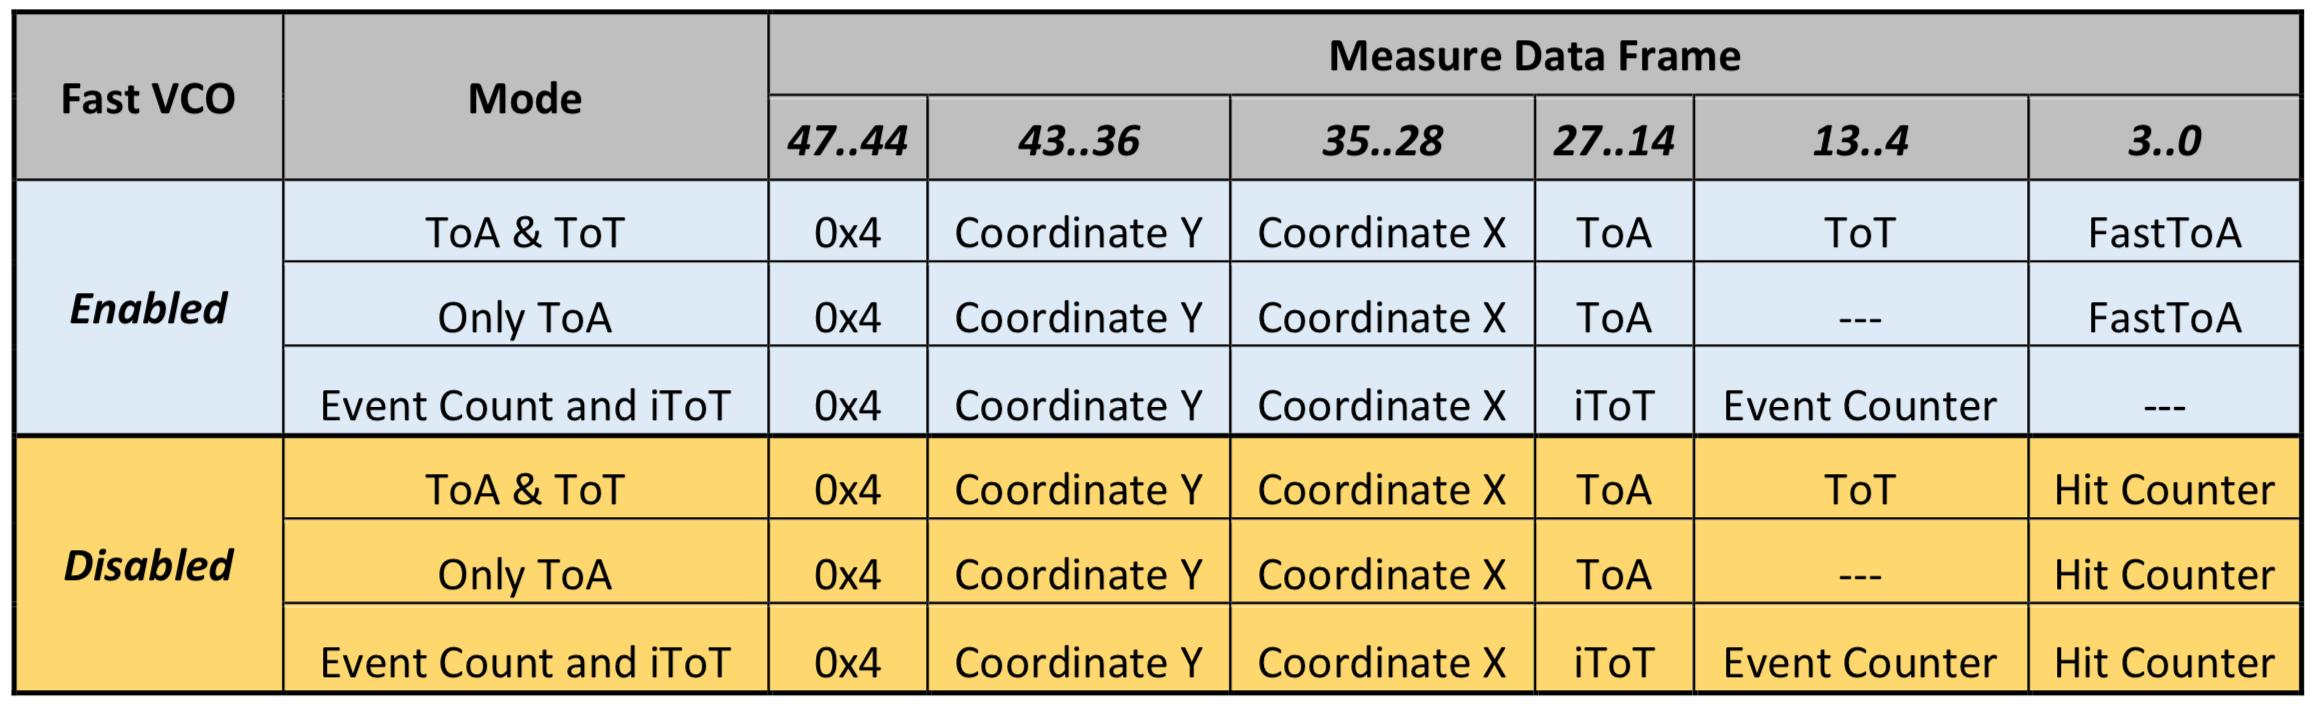
\includegraphics[width=14cm]{figures/katherine_pixel_measurement_data.png}
        \caption{Struktura měřených dat \cite{katherine_docs}.}
        \label{tab:katherine:protocol:measurement_data_structure}
    \end{center}
\end{table}



\section{Komunikační modul}\label{chap:katherine:comm}

\section{Datový modul}\label{chap:katherine:data}

\section{Katherine emulátor}\label{chap:katherine:emulator}